% SECTION ====================================================================================
\section{Natürliche Suchbäume}
% ============================================================================================

\begin{sectionbox}
\subsection{Nomenklatur}
\begin{center}
    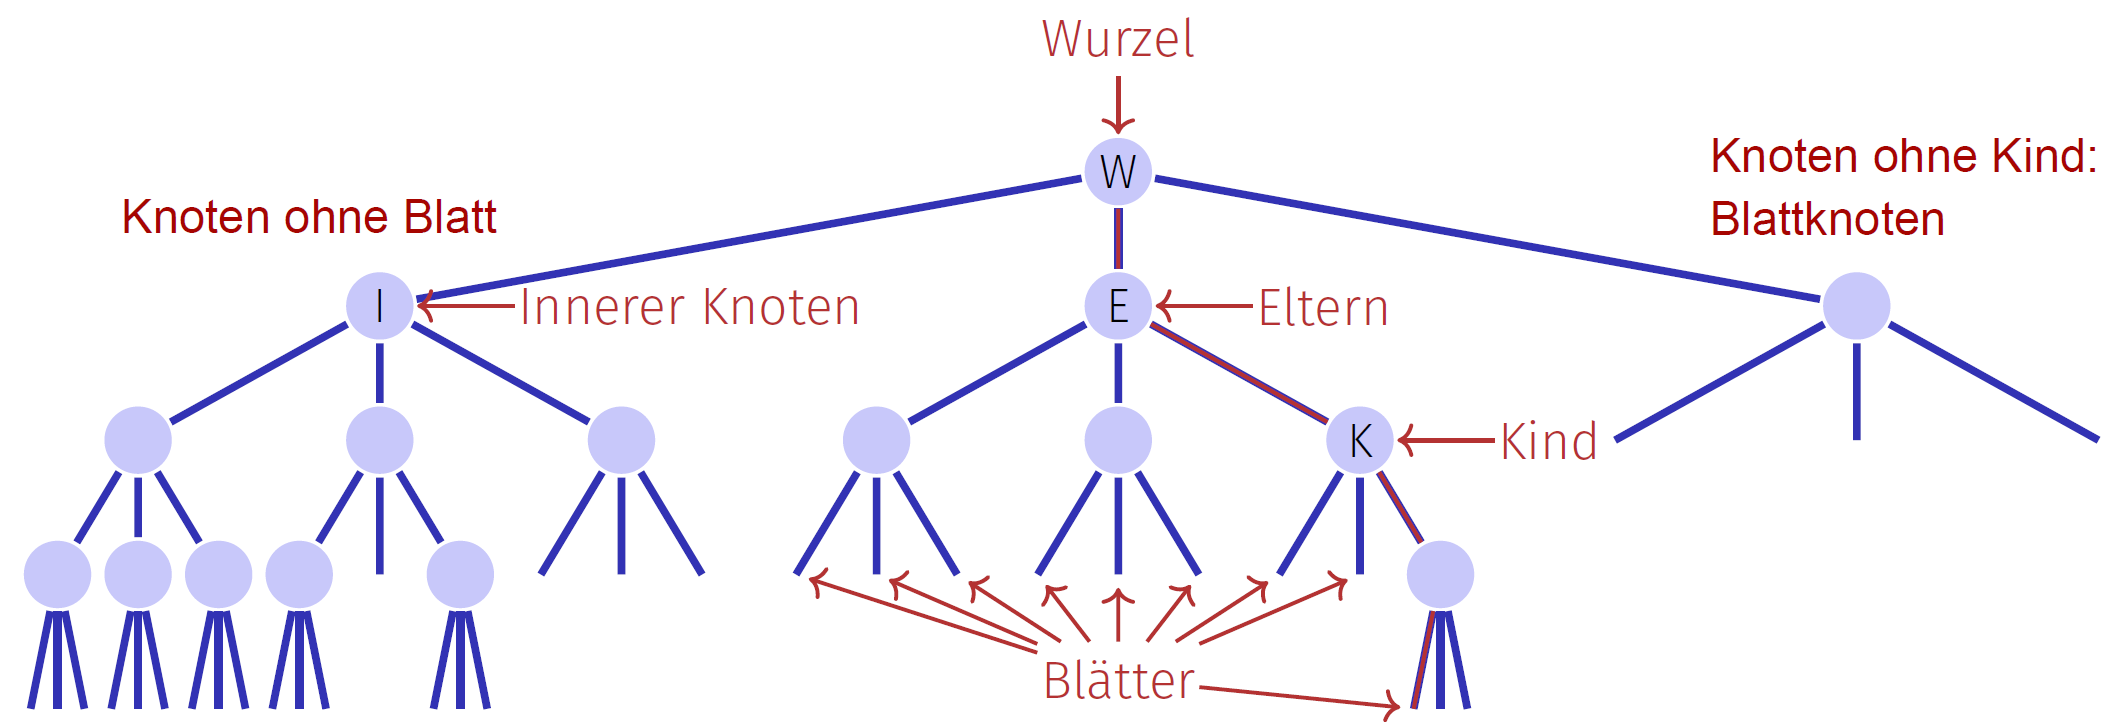
\includegraphics[width = \columnwidth]{../img/BaumNomen.png}
\end{center}
\end{sectionbox}

\begin{sectionbox}
\subsection{Binäre Suchbäume}\smallskip
Binärer Baum (nur zwei Nachfolgerknoten) mit Eigenschaten:\par
\begin{itemize}
    \item Jeder Knoten v speichert einen Schlüssel
    \item Schlüssel im linken Teilbaum v.left kleiner als v.key
    \item Schlüssel im rechten Teilbaum v.right grösser als v.key
\end{itemize}\vspace{7px}

\subsubsection{Höhe eines Baumes}\smallskip
$h(r)=\left\{\begin{array}{ll}0 & \text { falls } r=\text { null } \\ 1+\max \{h(r \cdot \operatorname{left}), h(r \cdot \text { right })\} & \text { sonst. }\end{array}\right.$\par\smallskip
Die Laufzeit der Suche ist somit im schlechtesten Fall $\mathcal{O}(h(T))$.\par\smallskip
\end{sectionbox}

\begin{sectionbox}
\subsubsection{Operationen}\smallskip
\textbf{Knoten suchen}\par\vspace{-4px}
\begin{lstlisting}[language=Python]
def search(k):
  global tree # access & modify the global variable tree
  v = tree
  while v != None:
    if k == v.key:
      return v
    elif k < v.key:
      v = v.left
    else:
      v = v.right
\end{lstlisting}

\textbf{Knoten einfügen}\par\vspace{-4px}
\begin{lstlisting}[language=Python]
def add(k):
  global tree # access & modify the global variable tree
  if tree is None:
    tree = Node(k)
    return True
  t = tree
  while k != t.key:
    if k < t.key:
      if t.left is None:
        t.left = Node(k)
        return True
      else:
        t = t.left
    else:
      if t.right is None:
        t.right = Node(k)
        return True
      else:
        t = t.right
  return False
\end{lstlisting}

\textbf{Knoten entfernen}\par
Mögliche Situationen: Knoten hat keine Kinder, Knoten hat ein Kind oder Knoten $v$ hat zwei Kinder.
Im letzten Fall: Der kleinste Schlüssel im rechten Teilbaum $v.right$ ist der symmetrische Nachfolger von $v$ $\rightarrow$ ersetze $v$ durch seinen symmetrischen Nachfolger.
\par Auch möglich: ersetze $v$ durch seinen symmetrischen Vorgänger
\par Implementation: der Teufel steckt im Detail!
\vspace{-4px}

\begin{lstlisting}[language=Python]
def remove(k):
  global tree # access & modify the global variable tree
  n = tree
  if n is not None and n.key == k:
    tree = symmetricDesc(tree)
    return True
  while n is not None:
    if n.left is not None and k == n.left.key:
      n.left = symmetricDesc(n.left)
      return True
    elif n.right is not None and k == n.right.key:
      n.right = symmetricDesc(n.right)
      return True
    elif k < n.key:
      n = n.left
    else:
      n = n.right
  return False
\end{lstlisting}

\textbf{Symmetrischen Nachfolger finden}\par\vspace{-4px}
\begin{lstlisting}[language=Python]
def symmetricDesc(node):
  if node.left is None:
    return node.right
  if node.right is None:
    return node.left
  n = node.right
  parent = None
  while n.left is not None:
    parent = n
    n = n.left
  if parent is not None:
    parent.left = n.right
    n.right = node.right
  n.left = node.left
  return n
\end{lstlisting}\vspace{-6px}

\end{sectionbox}

\begin{sectionbox}
\textit{Grafik zu dem symmetrischen Vorgänger (links) oder Nachfolger (rechts)}\par
\begin{center}
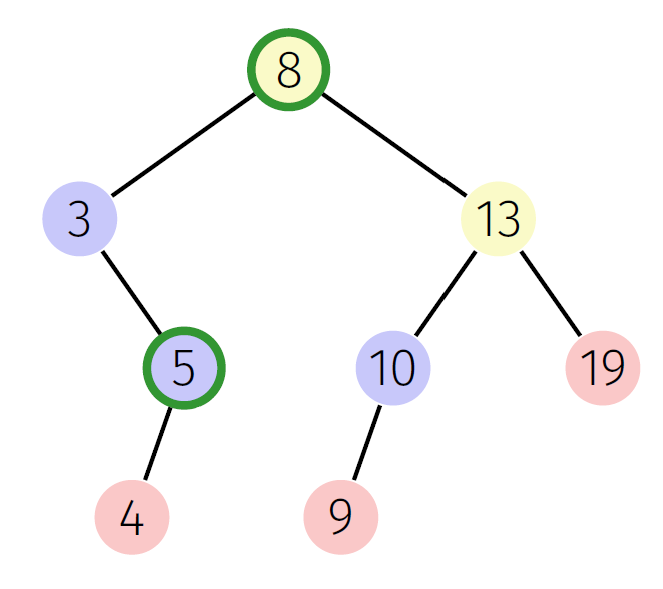
\includegraphics[width = 0.4\columnwidth]{../img/symVorg.png}
\tab 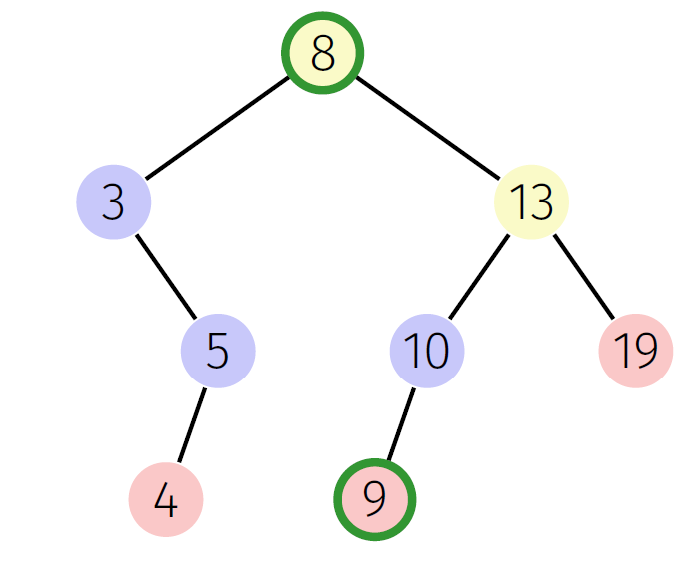
\includegraphics[width = 0.4\columnwidth]{../img/symNachf.png}    
\end{center}
\end{sectionbox}

\begin{sectionbox}
\subsection{Traversierungsarten}\smallskip
\begin{greenbox}
\begin{itemize}
    \item \textbf{Hauptreihenfolge} (preorder):
    \par $v$, dann $T_{left}(v)$, dann $T_{right}(v)$.
    \item \textbf{Nebenreihenfolge} (postorder):
    \par $T_{left}(v)$, dann $T_{right}(v)$, dann $v$.
    \item \textbf{Symmetrische Reihenfolge} (inorder):
    \par $T_{left}(v)$, dann $v$, dann $T_{right}(v)$.
\end{itemize}
\end{greenbox}\smallskip

\textit{Beispiel}\par
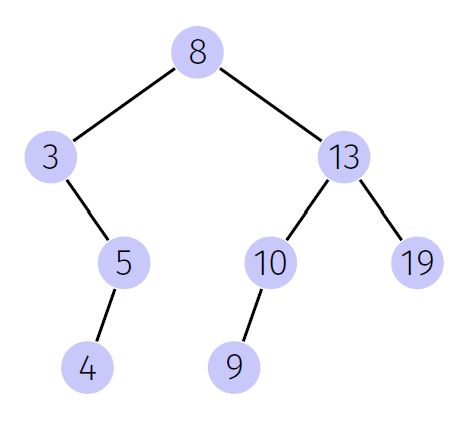
\includegraphics[width = 0.4\columnwidth]{../img/BspBST.png}
\smallskip
\begin{itemize}
    \item \textbf{Hauptreihenfolge} (preorder):
    \par 8, 3, 5, 4, 13, 10, 9, 19
    \item \textbf{Nebenreihenfolge} (postorder):
    \par 4, 5, 3, 9, 10, 19, 13, 8
    \item \textbf{Symmetrische Reihenfolge} (inorder):
    \par 3, 4, 5, 8, 9, 10, 13, 19
\end{itemize}

\end{sectionbox}
